\section{Impact of parameters on model predictions}
Here the impact of the parameters on the model predictions is shown. The most important parameters for the evolution of the infected population and the occurrence of the outbreak are $\beta$ and $\braket{k}$ parameters. The $\beta$ parameters is connected to the infection factor, so the probability of infecting a susceptible person in contact with and infected one. The $\braket{k}$ parameters indicate instead the number of connection for each individual, so measures the level of interaction of the Small-World. Since the two parameters always come together their effect is the same on the evolution and visible in Figure~\ref{fig:scan_i_vs_beta}, the larger those parameters are the steeper the curve of the infected population is, as expected from Equation~\ref{eqn:idot}.  A large impact on the outbreak evolution is also given by the fraction of quarantined infected population $\delta$, as shown in Figures~\ref{fig:scan_i_vs_delta} and \ref{fig:scan_q_vs_delta}. The outbreak is significantly contained in case a larger fraction of infected population is spotted and quarantined.

\begin{figure}[!ht]\centering
\subfloat[\label{fig:scan_i_vs_beta}]{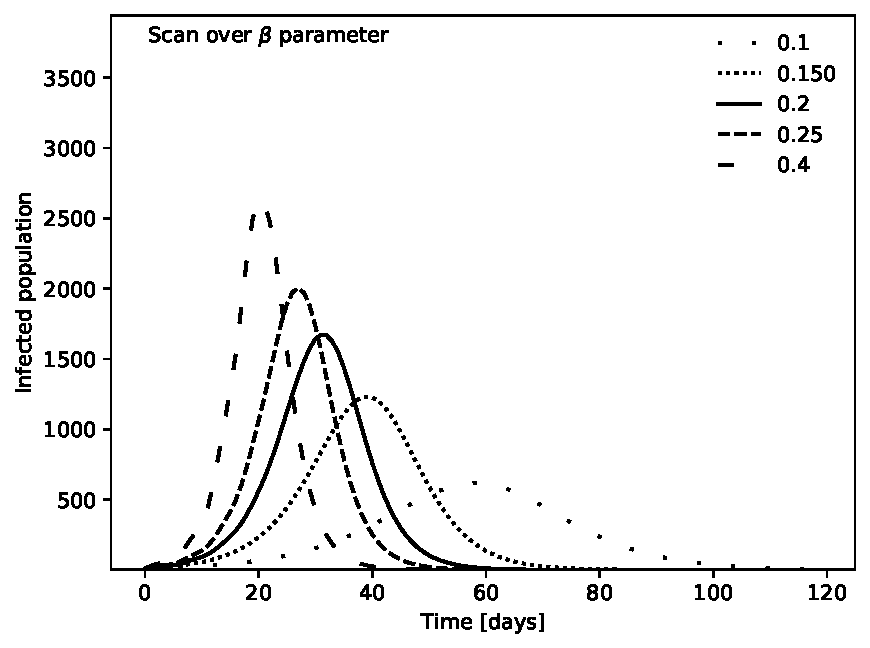
\includegraphics[width=0.32\textwidth]{imgs/ModelDescription/Scan_I_vs_beta_parameters_alternative.pdf}}
\subfloat[\label{fig:scan_i_vs_delta}]{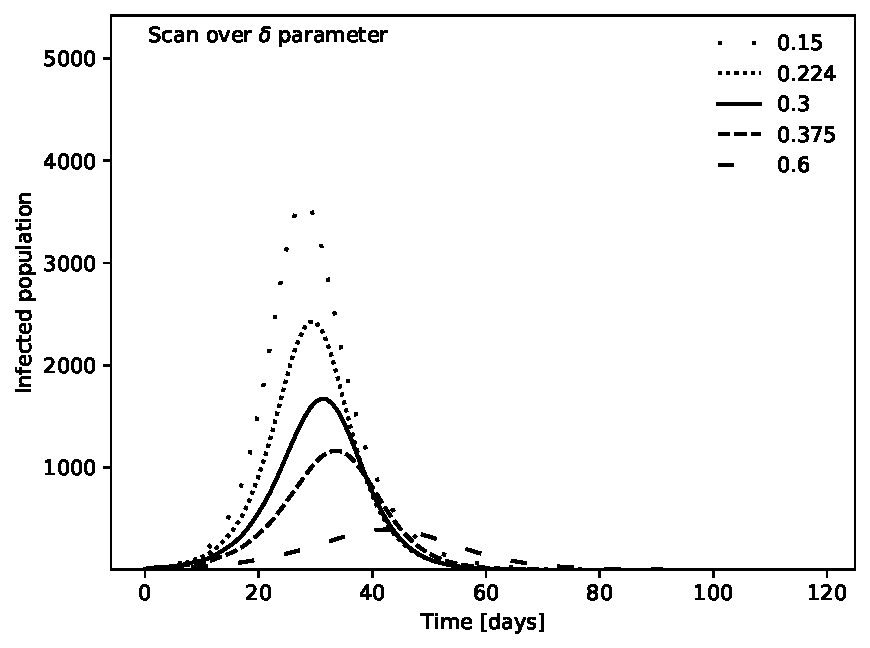
\includegraphics[width=0.32\textwidth]{imgs/ModelDescription/Scan_I_vs_delta_parameters_alternative.pdf}}
\subfloat[\label{fig:scan_q_vs_delta}]{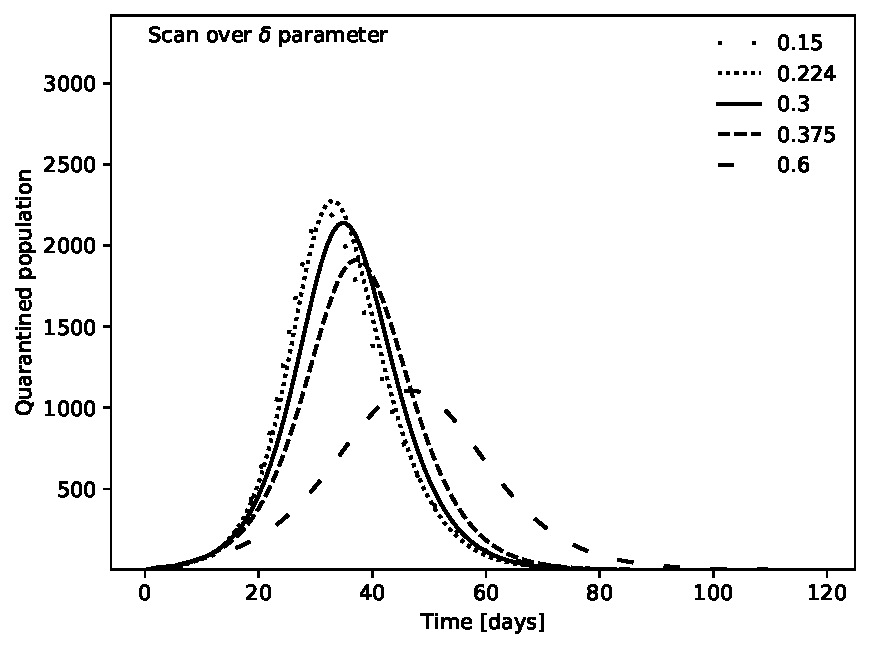
\includegraphics[width=0.32\textwidth]{imgs/ModelDescription/Scan_Q_vs_delta_parameters_alternative.pdf}}
\caption{Effect on the evolution of the infected population given by varying the $\beta$ parameter (a). Effect on infected (b) and quarantined (c) population given by varying the $\delta$ parameter.}.
\end{figure}

Other effects are given by $\gamma$, $\mu$ and $d_{1/2}$ parameters. Those control more the recovery curve. The $\gamma$ parameter is related to the probability of a recovered individual to not develop immunity: as shown in Figure~\ref{fig:scan_r_vs_gamma}, the recovered people has a decrease after the peak of the outbreak. The recovery curve is strongly affected by the $\mu$ parameter that regulates the recovery probability of the infected population, as shown in Figure~\ref{fig:scan_r_vs_mu}. The mortality $d_{1/2}$ instead increases the number of deaths, given by the difference of the recovered population and the initial $10000$ susceptible people, shown in Figure~\ref{fig:scan_r_vs_d1}.

\begin{figure}[!ht]\centering
\subfloat[\label{fig:scan_r_vs_gamma}]{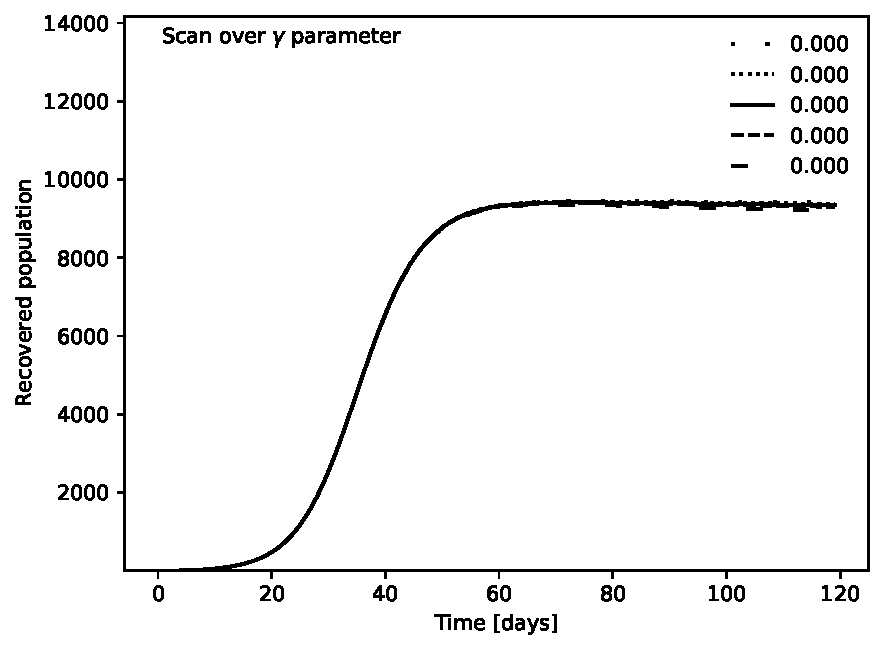
\includegraphics[width=0.32\textwidth]{imgs/ModelDescription/Scan_R_vs_gamma_parameters_alternative.pdf}}
\subfloat[\label{fig:scan_r_vs_mu}]{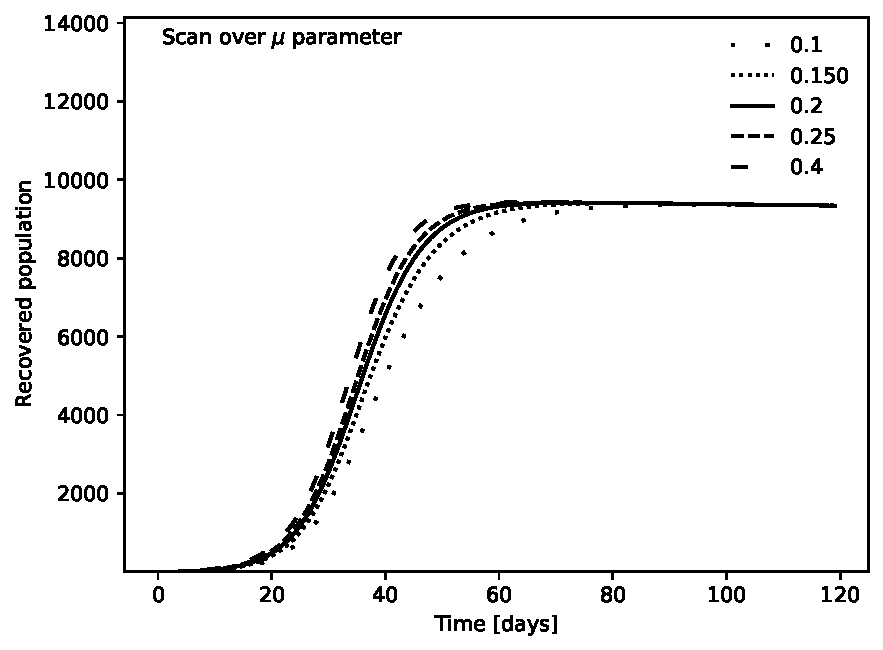
\includegraphics[width=0.32\textwidth]{imgs/ModelDescription/Scan_R_vs_mu_parameters_alternative.pdf}}
\subfloat[\label{fig:scan_r_vs_d1}]{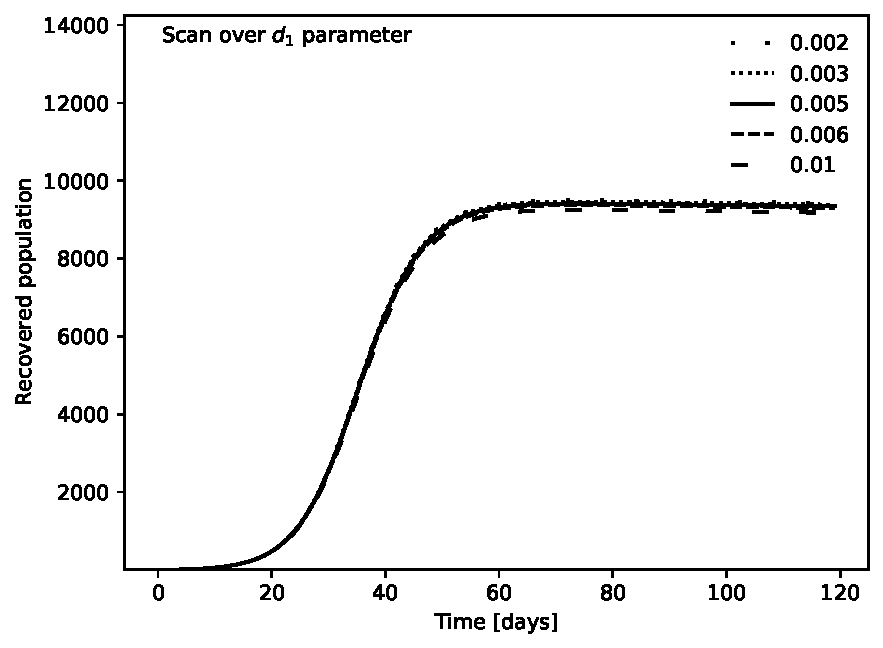
\includegraphics[width=0.32\textwidth]{imgs/ModelDescription/Scan_R_vs_d1_parameters_alternative.pdf}}
\caption{Effect on the evolution of the recovered population given by varying the $\gamma$ (a), $\mu$ (b) and $d_1$ (c) parameters.}.
\end{figure}

The only temporal parameter is the incubation time $\tau$: it also strongly affects the evolution of the oubreak, shown in Figure~\ref{fig:scan_i_vs_tau}. In case of long incubation time, the outbreak develops a  multiple peak structure, while in case of a short incubation time a clean ``gaussian'' peak is recognised.

\begin{figure}[!ht]\centering
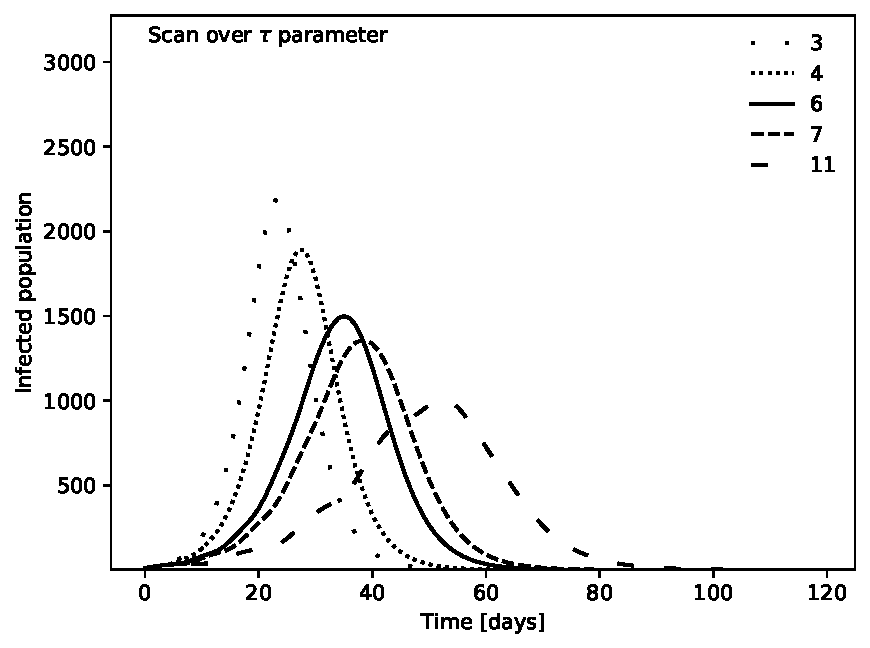
\includegraphics[width=0.4\textwidth]{imgs/ModelDescription/Scan_I_vs_tau_parameters_alternative.pdf}
\caption{Effect on the evolution of the infected population given by varying the $\tau$ parameter.}
\label{fig:scan_i_vs_tau}
\end{figure}
